\label{charged-Higgs}
Brandt and Hadavand will continue the search for charged Higgs in the fully hadronic final state of $\tau^+ \nu$.  The discovery of charged Higgs  would be a clear sign of BSM physics 
and would imply that the 125 GeV Higgs is part of a more complex Higgs sector. 
The Charged Higgs is predicted by several models such as ones with Higgs triplets and Two-Higgs-Doublet-Models(2HDM)~\cite{2hdm1,2hdm2,2hdm3}. 
%The observation of a charged Higgs would be a clear sign of BSM physics and would imply that the 125 GeV Higgs is part of a more complex Higgs sector. 
In the MSSM, which is a type II 2 Higgs Doublet Model (2HDM), the main production of charged Higgs at the LHC is t $\rightarrow$ b H$^+$ for H$^+$ mass below m$_{top}$. At charged Higgs masses above m$_{top}$
the main production at the LHC is in association with a top quark.  In the MSSM the Higgs sector can be completely determined by the H$^+$ mass and tan $\beta$, the ratio of vacuum expectation values of the 2HDM.
For masses below the top mass the $\tau \nu$ decay is dominant for $\tan \beta >2 $. 

%In Run 2 we expect that with only a few\invfb of data,
%We will have a much higher chance of seeing this final state due to the larger cross sections (10x in some cases) provided by the higher center of mass energy. The search with 3.2 \invfb of data at $\sqrt s$ = 13 TeV has been recently published ~\cite{taunu}.

Hadavand motivated and was responsible for investigating new models for analyzing the intermediate mass region of 160-180 GeV.
Only recently have theorists been able to reconcile \ttbar\ interference effects and supply the NLO calculations of the cross section as a function of mass and \tanb.
The addition of this mass region will close the gap m$_{H}$ vs \tanb\ mass range and also produce competitive results at low \tanb\ vs A $\rightarrow$ $\tau \tau$ and \Hp \too t$^+$b.  
The measurements for this region will be performed by the end of 2016.

Hadavand and Griffiths have led the charged Higgs as charged Higgs convener and analysis contact respectively.  Under their leadership UTA group has produced the final results including plots and statistical
interpretation, estimation of the systematic uncertainties, including theoretical, writing the analysis code, production of common ntuples, and trigger studies ( with Jae Yu's student Last Feremenga).  
%By using simulated \ttbar\ data instead of $\tau$ embedding~\cite{embedding} resulted in a paper with 3.2 \invfb\ of data and a conference note at 14.7\invfb\ of data at 13 TeV~\cite{taunu,hptnu1}.  
This luminosity increase extended the mass reach of the analysis from 250 GeV in Run 1 to 600 GeV in Run 2.
The jet to tau background statistics for the Run 2 analysis were vastly improved over Run 1 by using Hadavand's suggestion of only using a missing ET trigger as opposed to a tau plus missing ET trigger.  The use of the tau in the trigger implied that a medium selection of taus had to be used in the fake factor method, 
where in Run 2 a Loose selection could be used therefore greatly enhancing the statistics.

Figure~\ref{fig:tau} (middle) shows that with the 2018 dataset of 100-150 \invfb\ of data the analysis is excluding large \tanb\ values so this analysis continues to be an important measurement as more data in accumulated.
The group has plans to apply several techniques to improve the analysis sensitivity over it's early Run 2 predecessor.  The tasks aimed for these improvements are listed below:

%% HH fix analysis cuts
%{\it not sure if we need to detail the selection}
%\subsubsection{Selection and Backgrounds to \Hp $\tau\nu$}
%The selection for the \Hp analysis include the following 1.  ETmiss trigger, 2. $\tau$ with pT $> 40 $GeV, 3. At least 3 jets for heavy \Hp with pt $> 25$ GeV, 4. no electron or muon,
%5. ETmiss$ > 150(TBD)$ GeV for heavy(light) \Hp, 6.  at least 1(2) b tagged jet light(heavy).  The final discriminating variable used is 
%$m_T = \sqrt{ 2p^\tau_TE^{miss}_T(1-\cos {\Delta \phi_{\tau_{had-vis},miss}})}  $

%There are three major sources of background to the \Hp analysis.  They include 1. true $\tau$ background 2. QCD background 3. leptons faking $\tau$s.  1. and 2. were data driven for Run 1 while 3. is taken from MC simulations.  
%For the early Run 2 analysis only the QCD background was taken from data.  The other two backgrounds were derived from MC simulations. As a crosscheck, for the ICHEP 2016 results the shape of \ttbar\, true $\tau$ background was taken
%from MC while the normalization was taken from the fit to data.


\begin{figure}\label{fig:plot1}
\begin{center}
\includegraphics[height=0.27\textwidth]{Haleh/chargedHiggs-confnote-limits.eps}
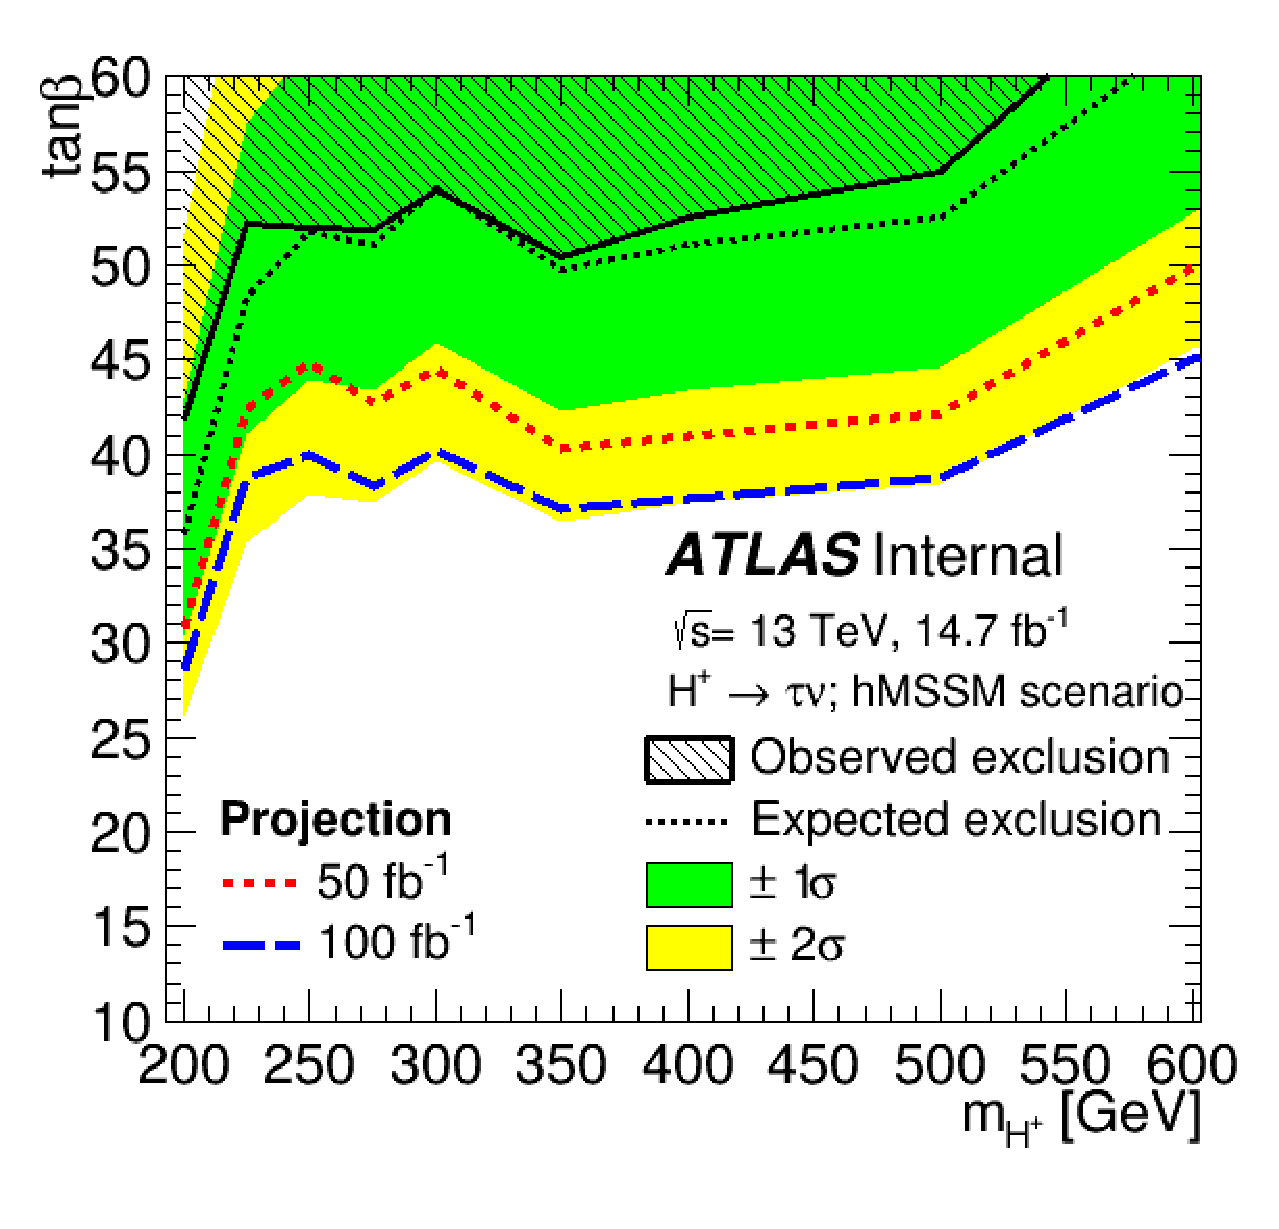
\includegraphics[height=0.27\textwidth]{Haleh/WithProjection_exclusion_run2016taunu_v2_hmssm_taunu.eps}
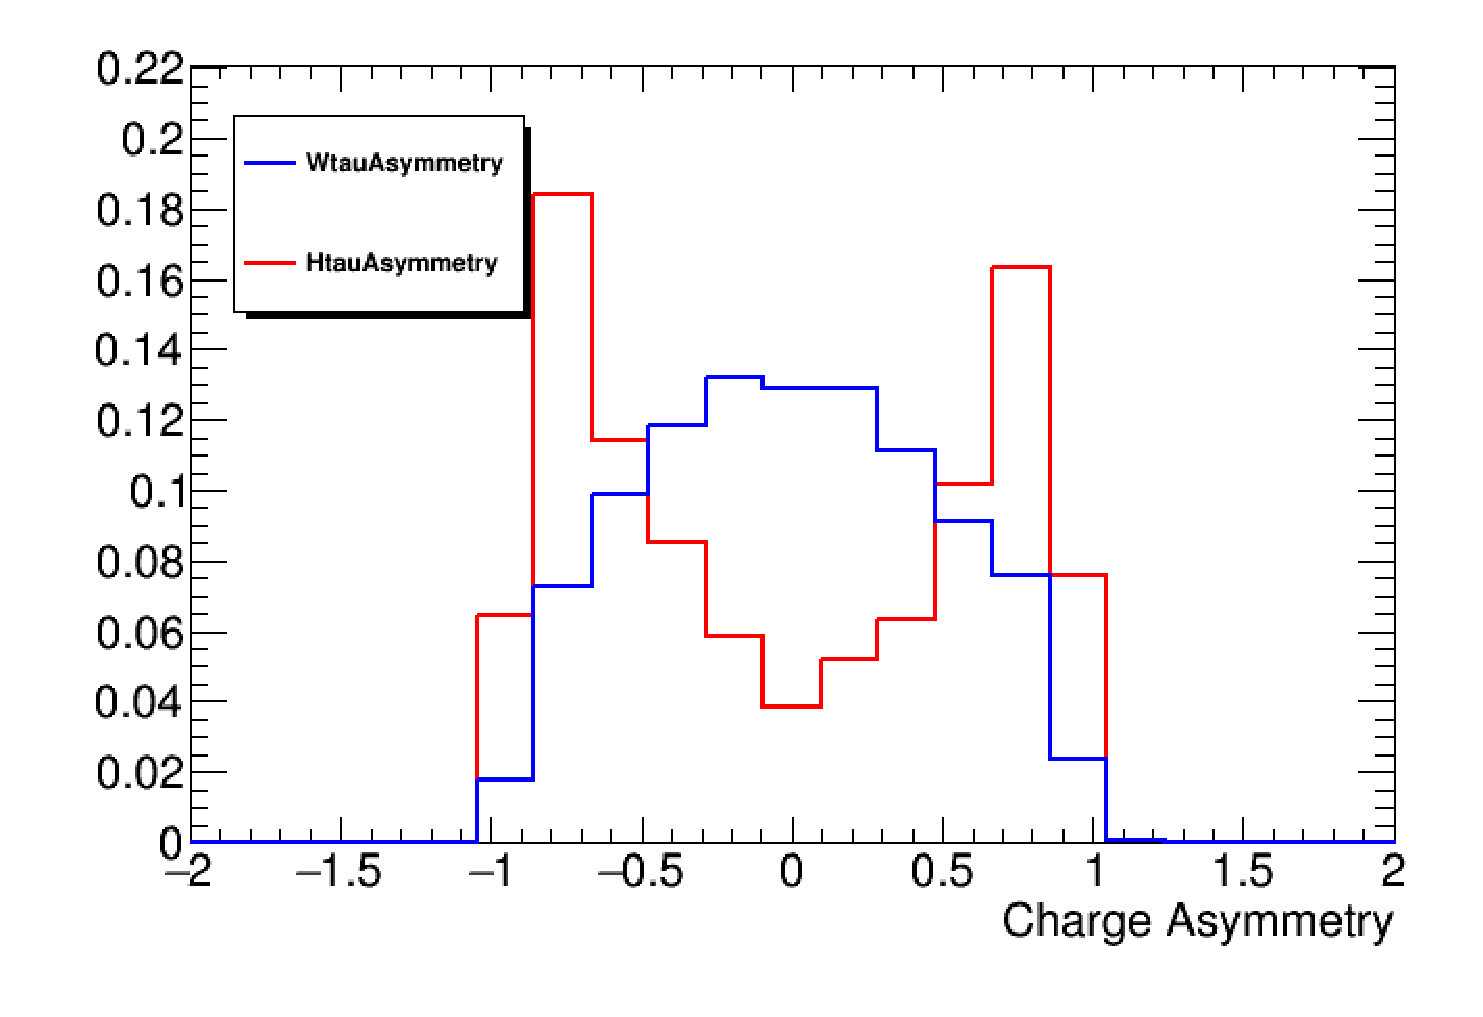
\includegraphics[height=0.25\textwidth, width=0.30\textwidth]{Haleh/tauAsy.eps}
\caption{ ICHEP 2016 hMSSM exclusions including 2015 exclusion, left; ICHEP 2016 hMSSM exclusions with 50\invfb\ and 100\invfb\ of data projections, middle; Distribution of $\tau$ polarization for Higgs and W decays, right;}
\label{fig:tau}
\end{center}
\end{figure}
\paragraph{Include tau-lep Channel}
By the end of 2016 the tau-lep channel (hadronic tau and leptonic top decays) will be added to the analysis.  This analysis will rely heavily on infrastructure used for the  tau hadronic final state developed by UTA 
for histogram production, systematic uncertainties, and limit setting. Therefore UTA will be an integral part of the addition of this final state.

\paragraph{Use tau polarization to reduce true tau background}
The tau polarization can be used to separate the W \too $\tau \nu$ background from the signal.  The intrinsic polarization of W$^+$ is -1 while that of $H^+$ is +1.  The tau polarization is defined as $P_{\tau}=\frac{\sigma_R - \sigma_L}{\sigma_R + \sigma_L}$.
A plot of the charge asymmetry, defined as $\Upsilon=\frac{p_{T}^{track}}{p_T} - 1$, is shown for the signal and background in the $\tau$ \too $\rho \nu_{\tau}$ final in figure~\ref{fig:tau}, right. Other 1-prong decays will also have similar separation in the charge asymmetry. 
The 1-prong decays can be separated from the 3-prong decays in the final fitting machinery and added statistically together.  This variable will be used as additional variable to the fit in the 1-prong case.

\paragraph{Use matrix element method to reduce true tau background}
In addition to the tau polarization one can utilize the event kinematics by utilizing the matrix element method to distinguish the signal from the true tau background originating from \ttbar\ events.  
This can be done by using the classifier distribution $d(x)=\frac{P_S(x)}{P_S(x)-P_B(x)}$ where $P_S$ and $P_B$ correspond to the weights from the signal and background 
hypothesis . Hadavand has performed initial tests with MadWeight for achieving this goal. This variable can then be added as one of the variables in the boosted decision trees (BDT). 

\paragraph{Use boosted decision trees}
As mentioned earlier for early Run 2 results the discriminating variable used in the fit was $m_T$. As an alternative several 
variables are incorporated into a BDT which is used as the discriminating variable in the fit.  Some variables that have been investigated in some preliminary studies
are $m_T$, leading b jet $p_T$ , $\tau p_T$, MET, $\Delta \eta(\tau-$leading jet), $\Delta \phi(top-$sub-leading jet).

\paragraph{Determine jet \too $\tau$ Background from Control Region}  %( R2-1, R3-1 - 3 months ) 
For Run 1 the systematics for the $\tau$ \too jet background were one the largest in the analysis.  Due to low statistics at the high mass a fit above 200 GeV was necessary to get 
an estimate of the background in that region.  This is important since this is the dominant background in the high mass region and without a background model the limit machinery would fail.
As an alternative to the matrix method used for the Run 1 published paper one can use a control region with no signal and loosen the selection criteria to introduce more fake taus.  This can be done
by requiring a zero b-jet region and only requiring a loose tau selection.  The normalization of this background can then be derived within the fit to data.  This should reduce both the statistical and systematic uncertainty of the analysis.
%In order to attain a control region with enough statistics when imposing this selection criteria one has to change the current trigger which already imposes a selection of a medium tau.  
%The use of the tau plus MET trigger has caused some of the main issues with statistics for the QCD background in Run 1. 
%Hadavand proposed to use a MET trigger which actually had higher efficiency than the tau plus MET trigger.  
%The use of this trigger increases the statistics for the background estimation.
%Other control region which are void of signal can be used in a similar fashion by fitting the normalization within the data.

\paragraph{Apply Deep learning techniques for selection}
The deep learning technique can be applied to this analysis in two ways.  One way would be to use it to distinguish \ttbar\ background from the signal by training on those samples.
A comparison of the BDT method described earlier for event selection will be done with respect to this technique.
Another way to apply deep learning would be in the tau reconstruction in place of the BDT technique which is used now.  This work will be done utilizing Farbin's extensive experience in the field of deep learning.


%\paragraph{Port Statistics Tool to new Naming Convention} ( R2-1 - 2 months )
%The statistics tools written for this analysis by myself and the UTA group have to be changed to accommodate the naming convention imposed by the new xAOD data format.  This will effect the systematic naming only.  It seems 
%like a trivial task but with around 70 nuisance parameters it can be quite tedious to implement.  Mr. Feremenga would benefit from doing this work so as to familiarize himself with the statistics framework of the analysis.

\paragraph{Optimize Binning for Limits} %( R2-1 - 2 months )
The low statistics in the tail of the mT distribution has made the H$^+$ \too $\tau \nu$ channel difficult for setting limits.  In many cases several systematic variations performed for pull determination would make the fits fail.  
This has to do with the fact that the data has low stats and is not smooth as opposed to MC samples which did have a smooth shape in the tail and could be fit successfully.
By making requirements on signal over background and the number of total background in a given
bin and then testing with pull estimation, Hadavand was able to optimize the best binning for both stability and sensitivity.  For performing projections to higher luminosities the background is extrapolated to higher masses
to determine a realistic scale of the background in this region. After performing the extrapolation the binning is re-optimized for the given luminosity projection, a technique developed by Hadavand.
\paragraph{Milestones}
\begin{itemize}[noitemsep,nolistsep]
\item{FY16 - Publish results for charged Higgs on 2016 dataset including the tau-lepton channel.}
\item{FY17 - Publish charged Higgs results using $\tau$ polarization.}
\item{FY17 - Hire new postdoc to work on charged Higgs and Z+X analyses.}
\item{FY18 - Charged Higgs results with Matrix Element Methods.}
\item{FY19 - Graduate student Akafzade graduates on charged Higgs analysis.}
\item{FY19 - Brandt student Crouch starts on analysis.}
\item{FY19 - Publish charged Higgs results using deep learning techniques for selection and/or tau reconstruction.}
\end{itemize}

%\paragraph{Perform Limit Calculations and Fit studies ;  Akafzade}% (R2-1, R3-1 - 1 months)
%At this point UTA has quite a bit of experience with the limit setting software. The machinery will be changed with respect to the early Run 2 measurements by adding 
%two categories, 1 prong and 3 prong tau decays.  The 1 prong tau decay channel will have an additional variable, the tau polarization variable.  This variable could be added to the BDT 
%but I believe one can gain more by using the shape as a pdf in the fit.
%Mr.  Akafzade should take over this machinery and be able to perform the final limits and also do the fit validation by making pull distributions for all the mass points.

%\paragraph{Perform Combination with direct and indirect Searches ;  Postdoc}% (R2-2, R3-1 - 1 months)
%For dataset R2-2 and R3-2 where we aim for a publication we can combine the results with direct decays of \Hp and indirectly through the neutral CP odd Higgs decays.  For direct searches we would combine \Hp \too $\tau \nu $ lepton final state where one will
%require an additional lepton from the top decay with the hadronic channel.  Combination with the \Hp to tb channel is not required since they cover unique regions in the \tanb\ vs mH plane. This combination will give limits within the \tanb\ and mA plane as well as \tanb\ and cos($\beta-\alpha$) plane. 
%One can also combine with indirect searches namely with A \too $\tau \tau$ and A \too Z h final states to make further exclusion over these two planes for various models.

%\paragraph{Perform Model Dependent Limits ;  Postdoc} %(R2-2, R3-1 - 1 months)
%After branching fraction and cross section limits are performed model dependent limits can be made to determine exclusions of certain models.  Models can include mhmax$\pm$, tauphobic, 2HDM Type III, Type IV, etc.  
